\documentclass[sigconf]{acmart}
\setlength{\paperheight}{11in}
\setlength{\paperwidth}{8.5in}

\usepackage{booktabs}
\usepackage{amsmath}
\usepackage{amssymb}
\newcommand{\R}{\mathbb{R}}

\newcommand{\calM}{\mathcal{M}}
\newcommand{\calV}{\mathcal{V}}
\newcommand{\calF}{\mathcal{F}}
\newcommand{\calH}{\mathcal{H}}

\newcommand{\bL}{\mathbf{L}}
\newcommand{\bV}{\mathbf{V}}
\newcommand{\bF}{\mathbf{F}}
\newcommand{\bR}{\mathbf{R}}
\newcommand{\bW}{\mathbf{W}}
\newcommand{\bM}{\mathbf{M}}
\newcommand{\bT}{\mathbf{T}}
\newcommand{\bv}{\mathbf{v}}
\newcommand{\bh}{\mathbf{h}}
\newcommand{\bK}{\mathbf{K}}
\newcommand{\bn}{\mathbf{n}}
\newcommand{\bd}{\mathbf{d}}
\newcommand{\bc}{\mathbf{c}} 
\newcommand{\bx}{\mathbf{x}} 
\newcommand{\ba}{\mathbf{a}}
\newcommand{\bb}{\mathbf{b}} 
 
\DeclareMathOperator*{\argmin}{arg\,min} % Jan Hlavacek
\graphicspath{ {./assets/} }


\setcopyright{rightsretained}
 
\begin{document}
\title{3D Printing Support Reduction via Skinning Deformation}
\subtitle{Extended Abstract}

\author{Julia Gilenko}
\affiliation{%
  \institution{University of Toronto}
} 
\email{julia.gilenko@mail.utoronto.ca}

\author{Peiqi Wang}
\affiliation{%
  \institution{University of Toronto}
}
\email{pq.wang@mail.utoronto.ca}

\author{Jiayi Eris Zhang}
\affiliation{%
  \institution{University of Toronto}
}
\email{jiayieris.zhang@mail.utoronto.ca}

% The default list of authors is too long for headers.
\renewcommand{\shortauthors}{Julia G. Mark W. Eris Z.}

\begin{abstract}
 
In layer-based 3D fabrication, supporting materials are fabricated to support overhanging regions yet discarded later. Reducing supports saves both time and material cost. In this abstract, we propose a skeleton-based deformation method that slims down the supporting structure. We achieve this by searching globally in the space of linear blending transformations on skeleton handles, making a trade-off among as-rigid-as-possible, overhang, and self-intersection energies. Beyond minimizing supports, our method generates semantically meaningful deformation while avoiding artifacts e.g. self-intersection. This approach could be generalized to include arbitrary constraints by incorporating additional objectives, such as the center of mass for balancing and physical properties of printing material for self-support. With precomputed bounded biharmonic weights, our method has the potential to be GPU accelerated and employed as a real-time user interface that helps model design and fabrication.\footnote{Code is available at https://github.com/tt6746690/fast\_support\_reduction}
\end{abstract}

%
% The code below should be generated by the tool at
% http://dl.acm.org/ccs.cfm
% Please copy and paste the code instead of the example below.
%
\begin{CCSXML}
    <ccs2012>
    <concept>
    <concept_id>10010147.10010371.10010396.10010398</concept_id>
    <concept_desc>Computing methodologies~Mesh geometry models</concept_desc>
    <concept_significance>300</concept_significance>
    </concept>
    </ccs2012>
\end{CCSXML}

\ccsdesc[300]{Computing methodologies~Mesh geometry models}

\keywords{geometry processing, shape deformation, 3D fabrication}

\begin{teaserfigure}
    \centering
    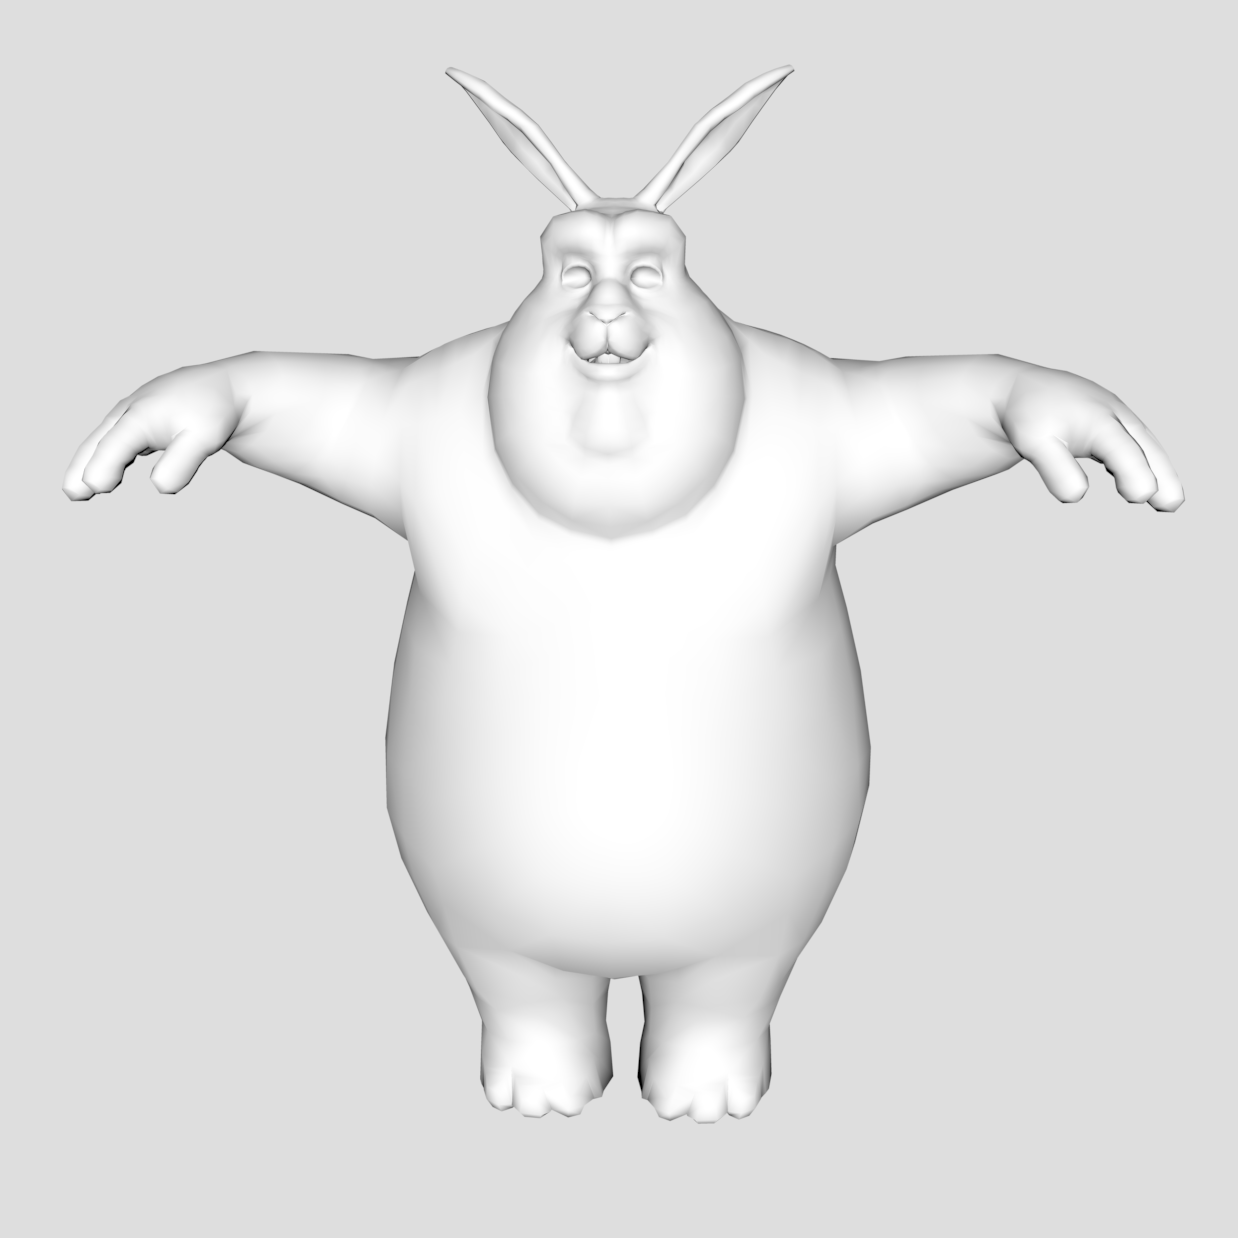
\includegraphics[width=0.13\textwidth]{bb_bunny.png} 
    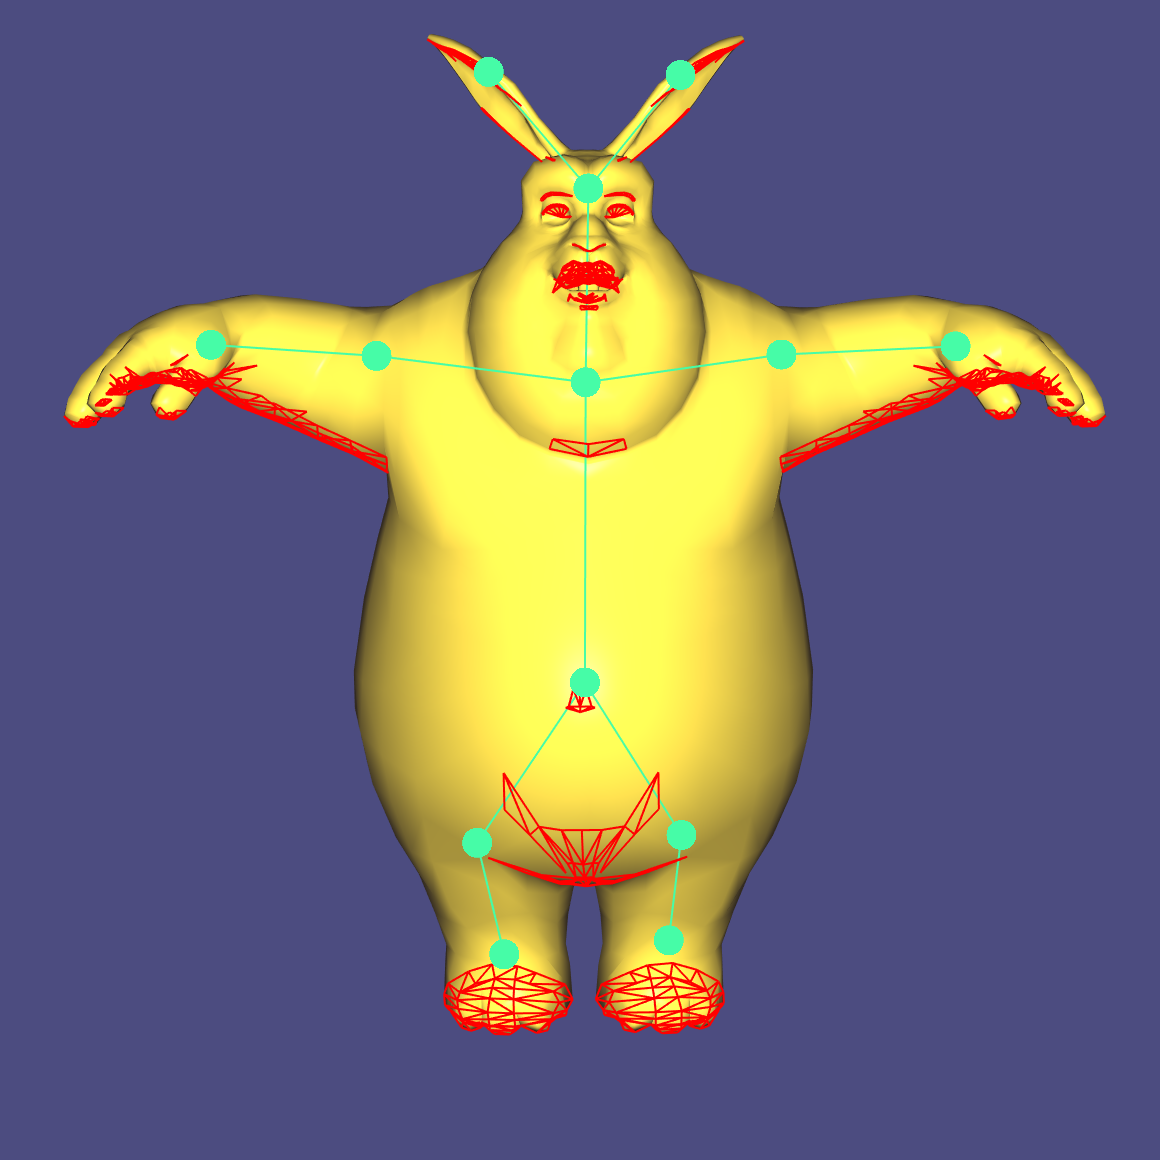
\includegraphics[width=0.13\textwidth]{bb_bunny_igl.png} 
    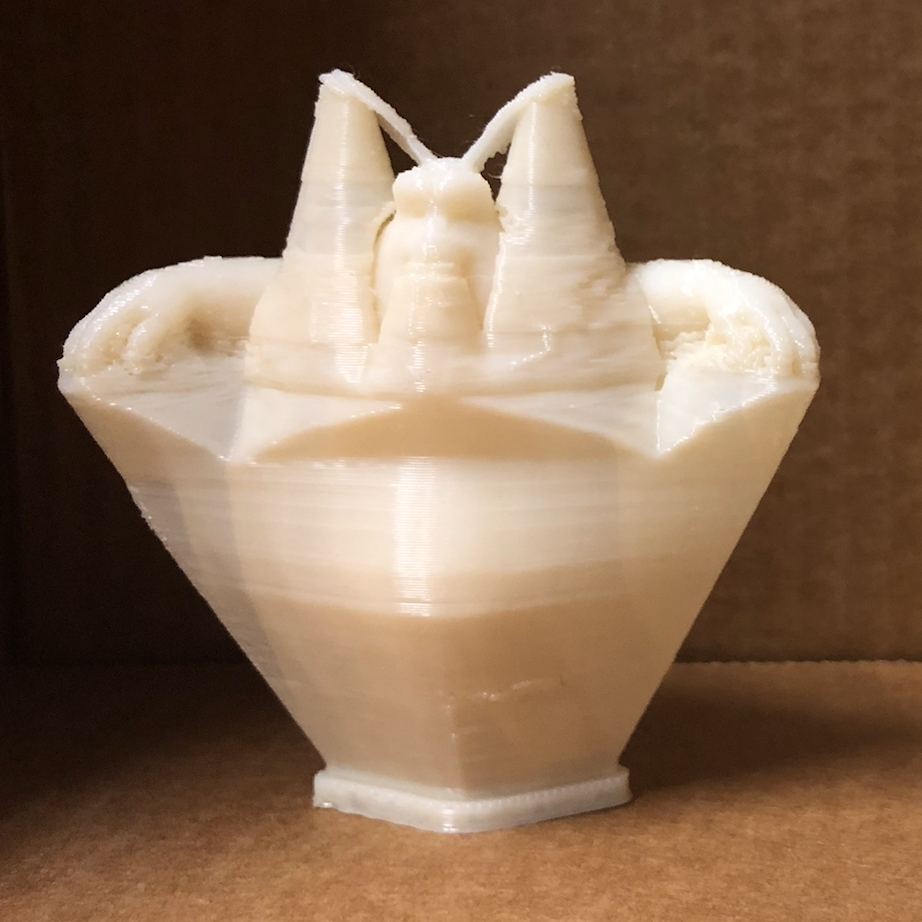
\includegraphics[width=0.13\textwidth]{bb_bunny_3dp.png}
    \quad
    {\LARGE$\rightarrow$}
    \quad
    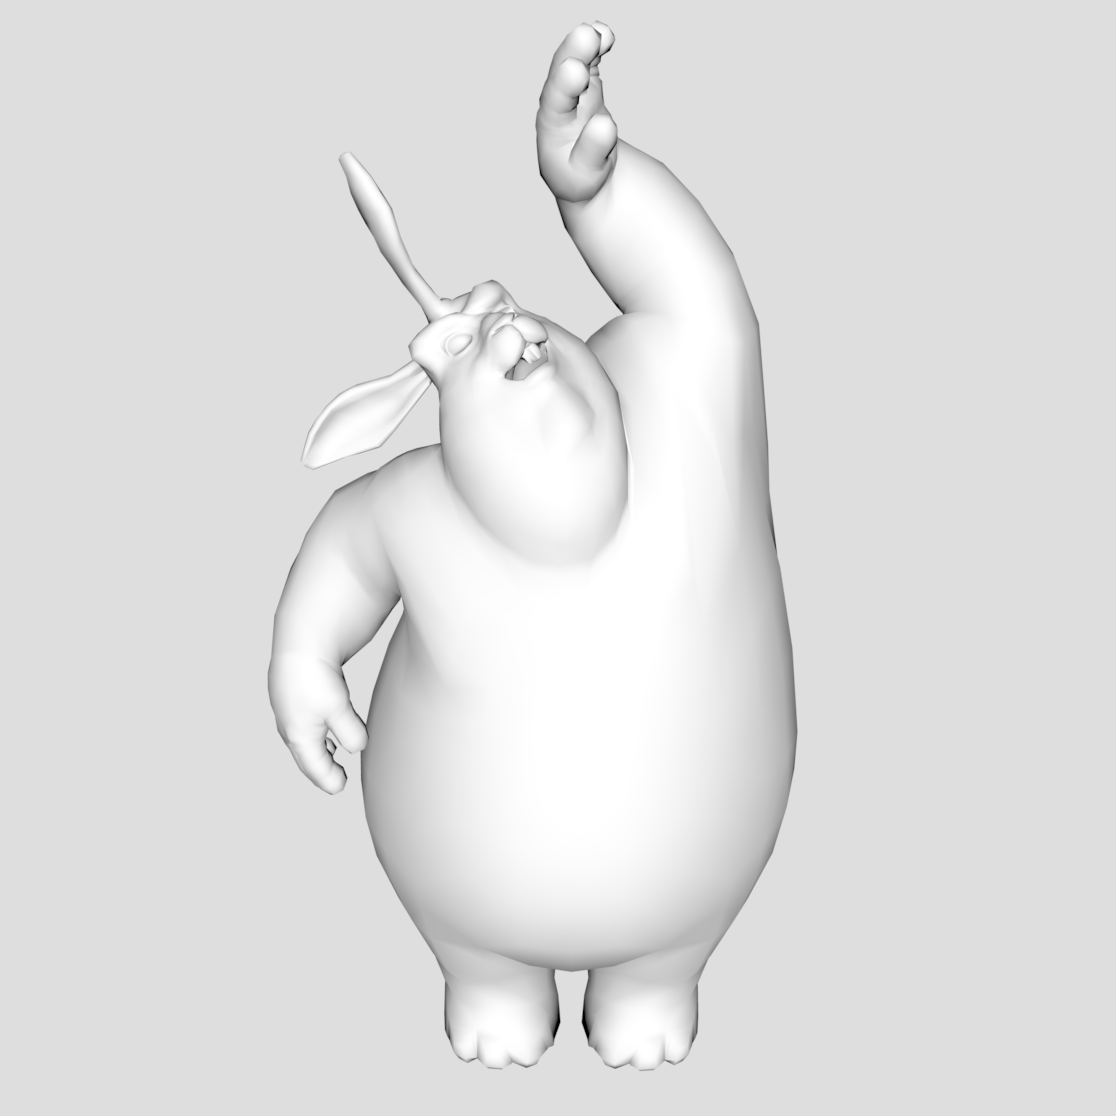
\includegraphics[width=0.13\textwidth]{bb_bunny_deformed.png} 
    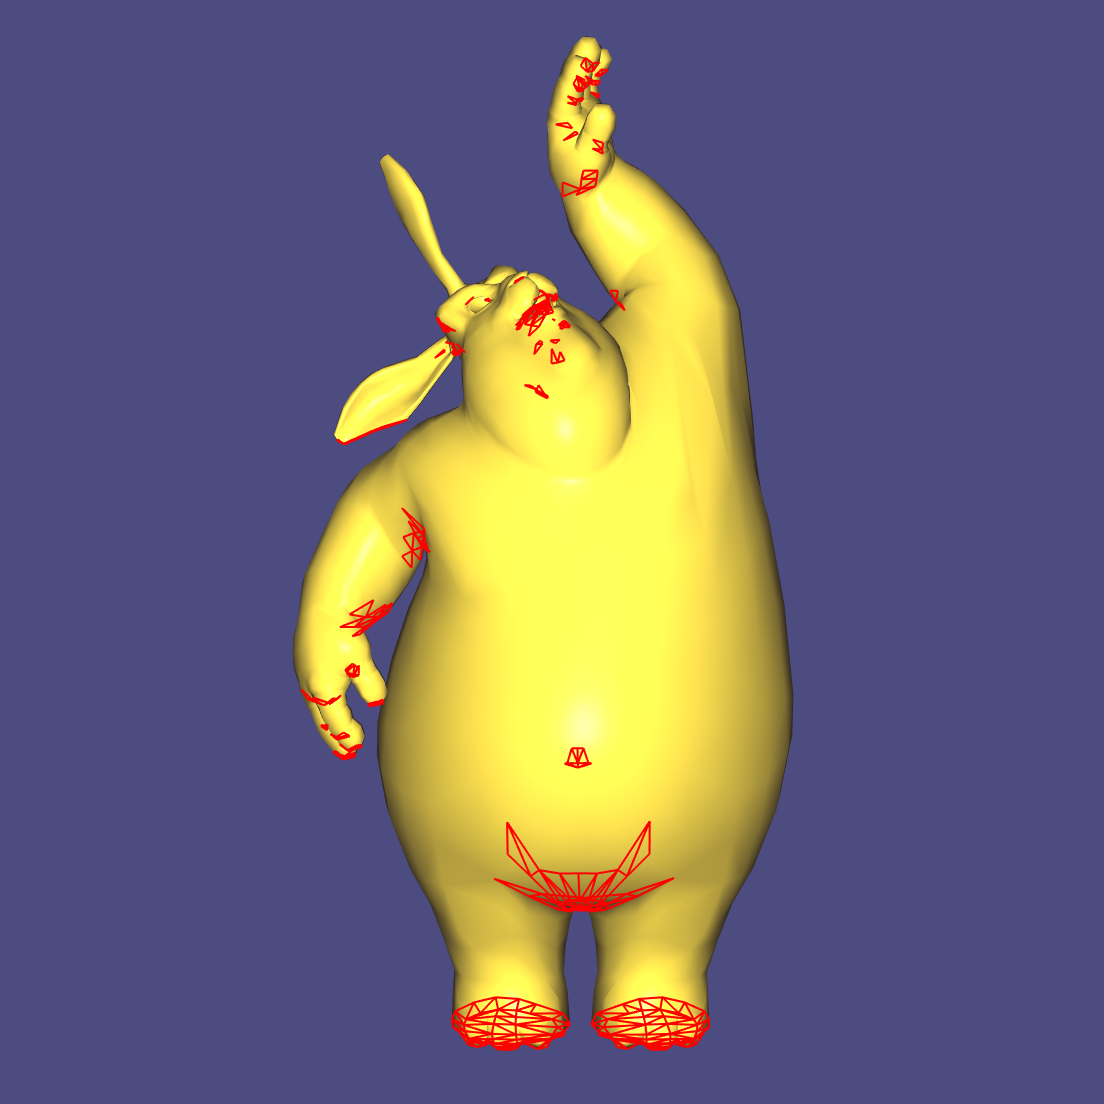
\includegraphics[width=0.13\textwidth]{bb_bunny_deformed_igl.png} 
    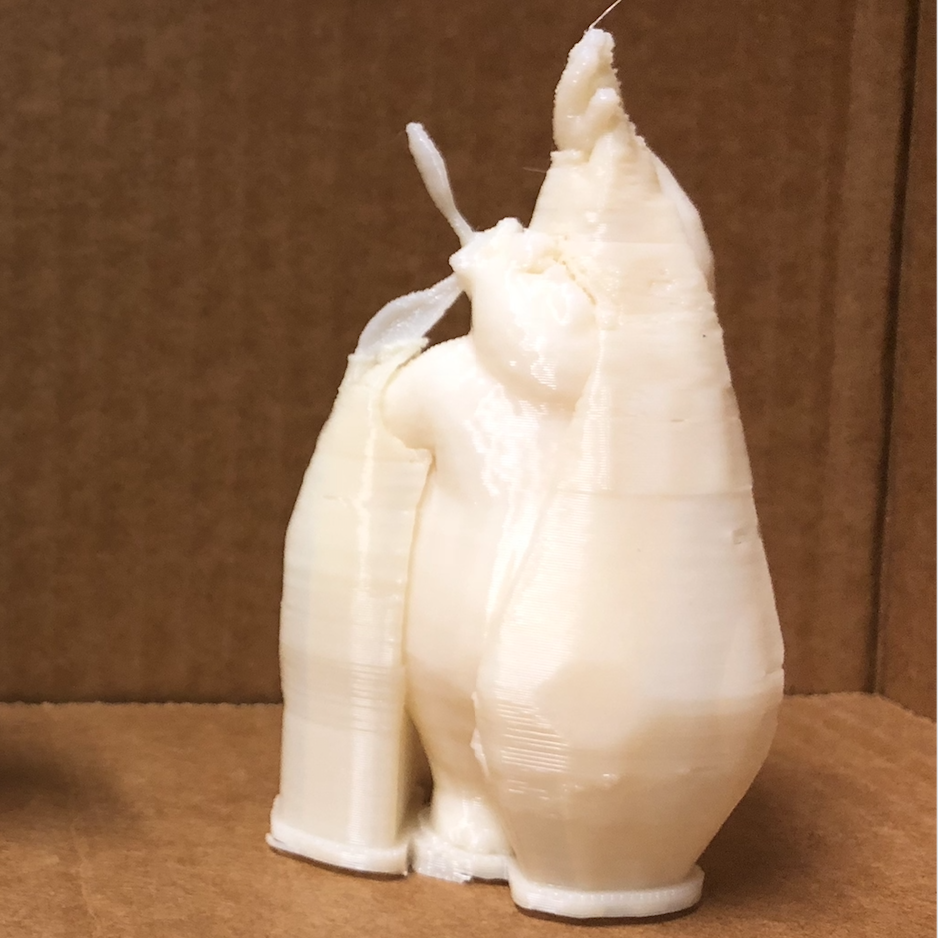
\includegraphics[width=0.13\textwidth]{bb_bunny_deformed_3dp.png}
    \caption{Our method generates natural skinning deformation with reduced support structures}
    \label{fig:bb_bunny}
\end{teaserfigure}

\maketitle



\subsection*{Introduction}


 
When a model needs supports in order to be 3D printed, the printer must use extra material, which makes printing more expensive. Existing work on the problem of how to reduce supports focusses predominantly on how to print support the same areas using less material. However, if the user is not particular about how the model is positioned when it is printed, there may also be a deformation that would require fewer supports. Given a skeleton for the model, we suggest a method to find a deformation using linear blend skinning to minimize the number of supports the model would need to be printed.

\subsubsection*{Problem formulation}
Let $\calM = (\bV, \bF)$ be a mesh living in dimension $d\in \{2,3\}$. Let $\bV = \{\bv_1^T, \cdots, \bv_n^T\}^T \in \R^{n \times d}$ be the rest-pose vertex positions. Given a set of control handles $\calH = \{ \bh_1, \cdots, \bh_m \}$, we can apply an affine transformation $\bT_j \in \R^{d \times (d+1)}$ on each handle $\bh_j$. Let $\bT = \{ \bT_1^T, \cdots, \bT_m^T \}^T \in \R^{(d+1)m \times d}$. Linear blend skinning is a deformation method whereby the positions of the vertices $\bV'$ on the deformed shape are calculated with a weighted linear combination of the handles' transformations,
\[
    \bv_i' = \sum_{j=1}^m w_j(\bv_i) \bT_j 
    \begin{pmatrix} 
    \bv_i \\
    1 
    \end{pmatrix} 
\]
where $w_j: \calM \rightarrow \R$ is computed using bounded biharmonic weights. Equivalently, $\bV' = \bM \bT$, where $\bM \in \R^{n \times (d+1)m}$ is a matrix combining $\bV$ and $\bW$. Note that the energies below are a function of $\bV'$, and hence a function of $\bT$ if we substitute $\bM \bT$ in its place, i.e. 
\[
    E_{arap}(\bT) = E_{arap}(\bT, \bM) = E_{arap}(\bV')
\]
where $\bM$ is fixed.

\subsection*{Energy terms} 

\subsubsection*{ARAP energy}

We can define the \textit{as-rigid-as-possible} deformation energy, which measures local distortion, to be
\[
    E_{arap}(\bV', \bR) = \frac{1}{2} \sum_{f\in \bF} \sum_{(i,j)\in f} c_{ij} || (\bv_i' - \bv_j') - \bR(\bv_i - \bv_j) ||^2
\]
Reformulating the ARAP energy to be a function of $\bV'$ only, we get
\[
    E_{arap}(\bV')
    \qquad
    \bR = \argmin_{\bR} tr(\bR\tilde{\bK}\bT)
\]
In matrix form, this becomes
\begin{align*}
E_{arap}(\bV') 
    &= tr(\frac{1}{2}\bV'^T \bL \bV' + \bV'^T \bK \bR ) \\
    &= tr(\frac{1}{2}\bT^T \tilde{\bL} \bT + \bT^T \tilde{\bK} \bR)
\end{align*}
    
where $\tilde{\bL} = \bM^T \bL \bM \in \R^{(d+1)m \times (d+1)m}$, $\tilde{\bK} = \bM^T \bK \in \R^{(d+1)m \times dn}$ and $\bK$ as defined in the deformation assignment

\subsubsection*{Overhang energy}

An overhanging region that can be 3D printed without support is called \textit{self-supported}. We call the angle between the region's tangent plane and printing direction the \textit{self-supported angle} $\alpha$. Let $\alpha_{max}$ be the maximum supporting angle. Let $\tau = cos(\alpha_{max})$ be the \textit{maximal supporting coefficient}. Let $\partial \calM \subset \bF$ be boundary of mesh $\calM$, i.e. surface faces. A surface face $f$ is \textit{risky} and thus requires support if $\bn_f \cdot \bd_{p} < -\tau$, where $\bn_f$ is unit normal of $f$ and $\bd_{p}$ is the printing direction. Let $A(\cdot)$ the area function and $c(\cdot)$ be the centroid function for a face $f$. We can approximate the volume of support required for any face $f$ by computing the volume of a rectangular prism,
\[
    \lambda(f) = 
    \begin{cases}
        A_{base} h = A_f |\cos(\theta_f)| (\bc_f \cdot \bd_{p}) = A_f |\bn_f \cdot \bd_{p}| (\bc_f \cdot \bd_{p}) & \text{if } \bn(f) \cdot \bd_{p} < -\tau \\
        0 & otherwise \\
    \end{cases}
\]
where $A_f$ is the area of the face, $\bc_f$ is the centroid of the face, and $\theta_f$ is the angle between $\bd_{p}$ and $\bn_f$. We define an overhang energy that measures the volume of support required,
\[
    E_{overhang}(\bV') = \sum_{f\in \partial \calM} \lambda(f)
\]
% \[
%     E_{overhang}(\bV') = \sum_{f\in \partial \calM} min(\bn(f) \cdot \bd_{p} + \tau, 0)
% \]


\subsubsection*{Self-intersection energy}

To prevent ARAP from deforming the mesh in such a way as to cause self-intersections, we add a third energy to measure them. We define a \textit{self-intersecting region} as the region inside the mesh that is bordered by intersecting tetrahedra. Given $j$ such regions we define the self-intersection energy to be
\[
	E_{intersect}(\bV') = \sum_{i=1}^j V_i
\]

where $V_i$ is the volume of the $i^{\text{th}}$ region. To find these volumes, we define a grid below the mesh and trace a ray up from every grid point. If it enters the mesh twice in a row, we know the ray must be in a self-intersecting region. "Entering" simply means the direction of the ray is opposite to the vertical component of the normal direction of the surface at that point. When it exits this region, we record the distance the ray traversed inside it. The sum of all these lengths produces an approximation of the combined volume. The finer the grid, the more accurate the approximation.


\subsection*{Optimization}

We define an objective function $E(\bx): \R^n \rightarrow \R$ as the sum of the three energy terms $E = E_{arap} + E_{overhang} + E_{intersect}$
and minimize $E$ using the particle swarm optimization. Let $\bx \in \R^{2dm}$ consisting a representation of centroid and rotation (as Euler's angle) about the centroid of for each edge handle. For shape in 

Finally, we can convert each component to $\bT_j$, affine transformations for edge handles, from which can compute deformed shaped $\bV' = \bM \bT$ with LBS.

\subsection*{Results?}

\subsection*{Future work}
In future work, we would like to speed up the calculations with a GPU. This would reduce wait time for the user and introduce the possibility of user interactivity, so that a user could have some control over the model's final position. We would also like to have the optimizer consider how the deformation shifts the model's center of mass, so that the model would still be able to stand on its own once it has been printed.
\newpage

\bibliographystyle{ACM-Reference-Format}
\bibliography{references}

\end{document} 
 
